\chapter{Предисловие}

\noindent
Совет ветеранов микрорайона, куда входит дом 2/6 по Хоромному тупику~-- Дом у Красных ворот, под руководством Т. В. Меньшиковой, которая продолжает дело своего отца, ведет подготовку к выпуску памятного альбома, посвященного истории и людям этого дома.

\vspace{10pt}

\begin{figure}[ht]
  \centering
  \begin{minipage}{7cm}
  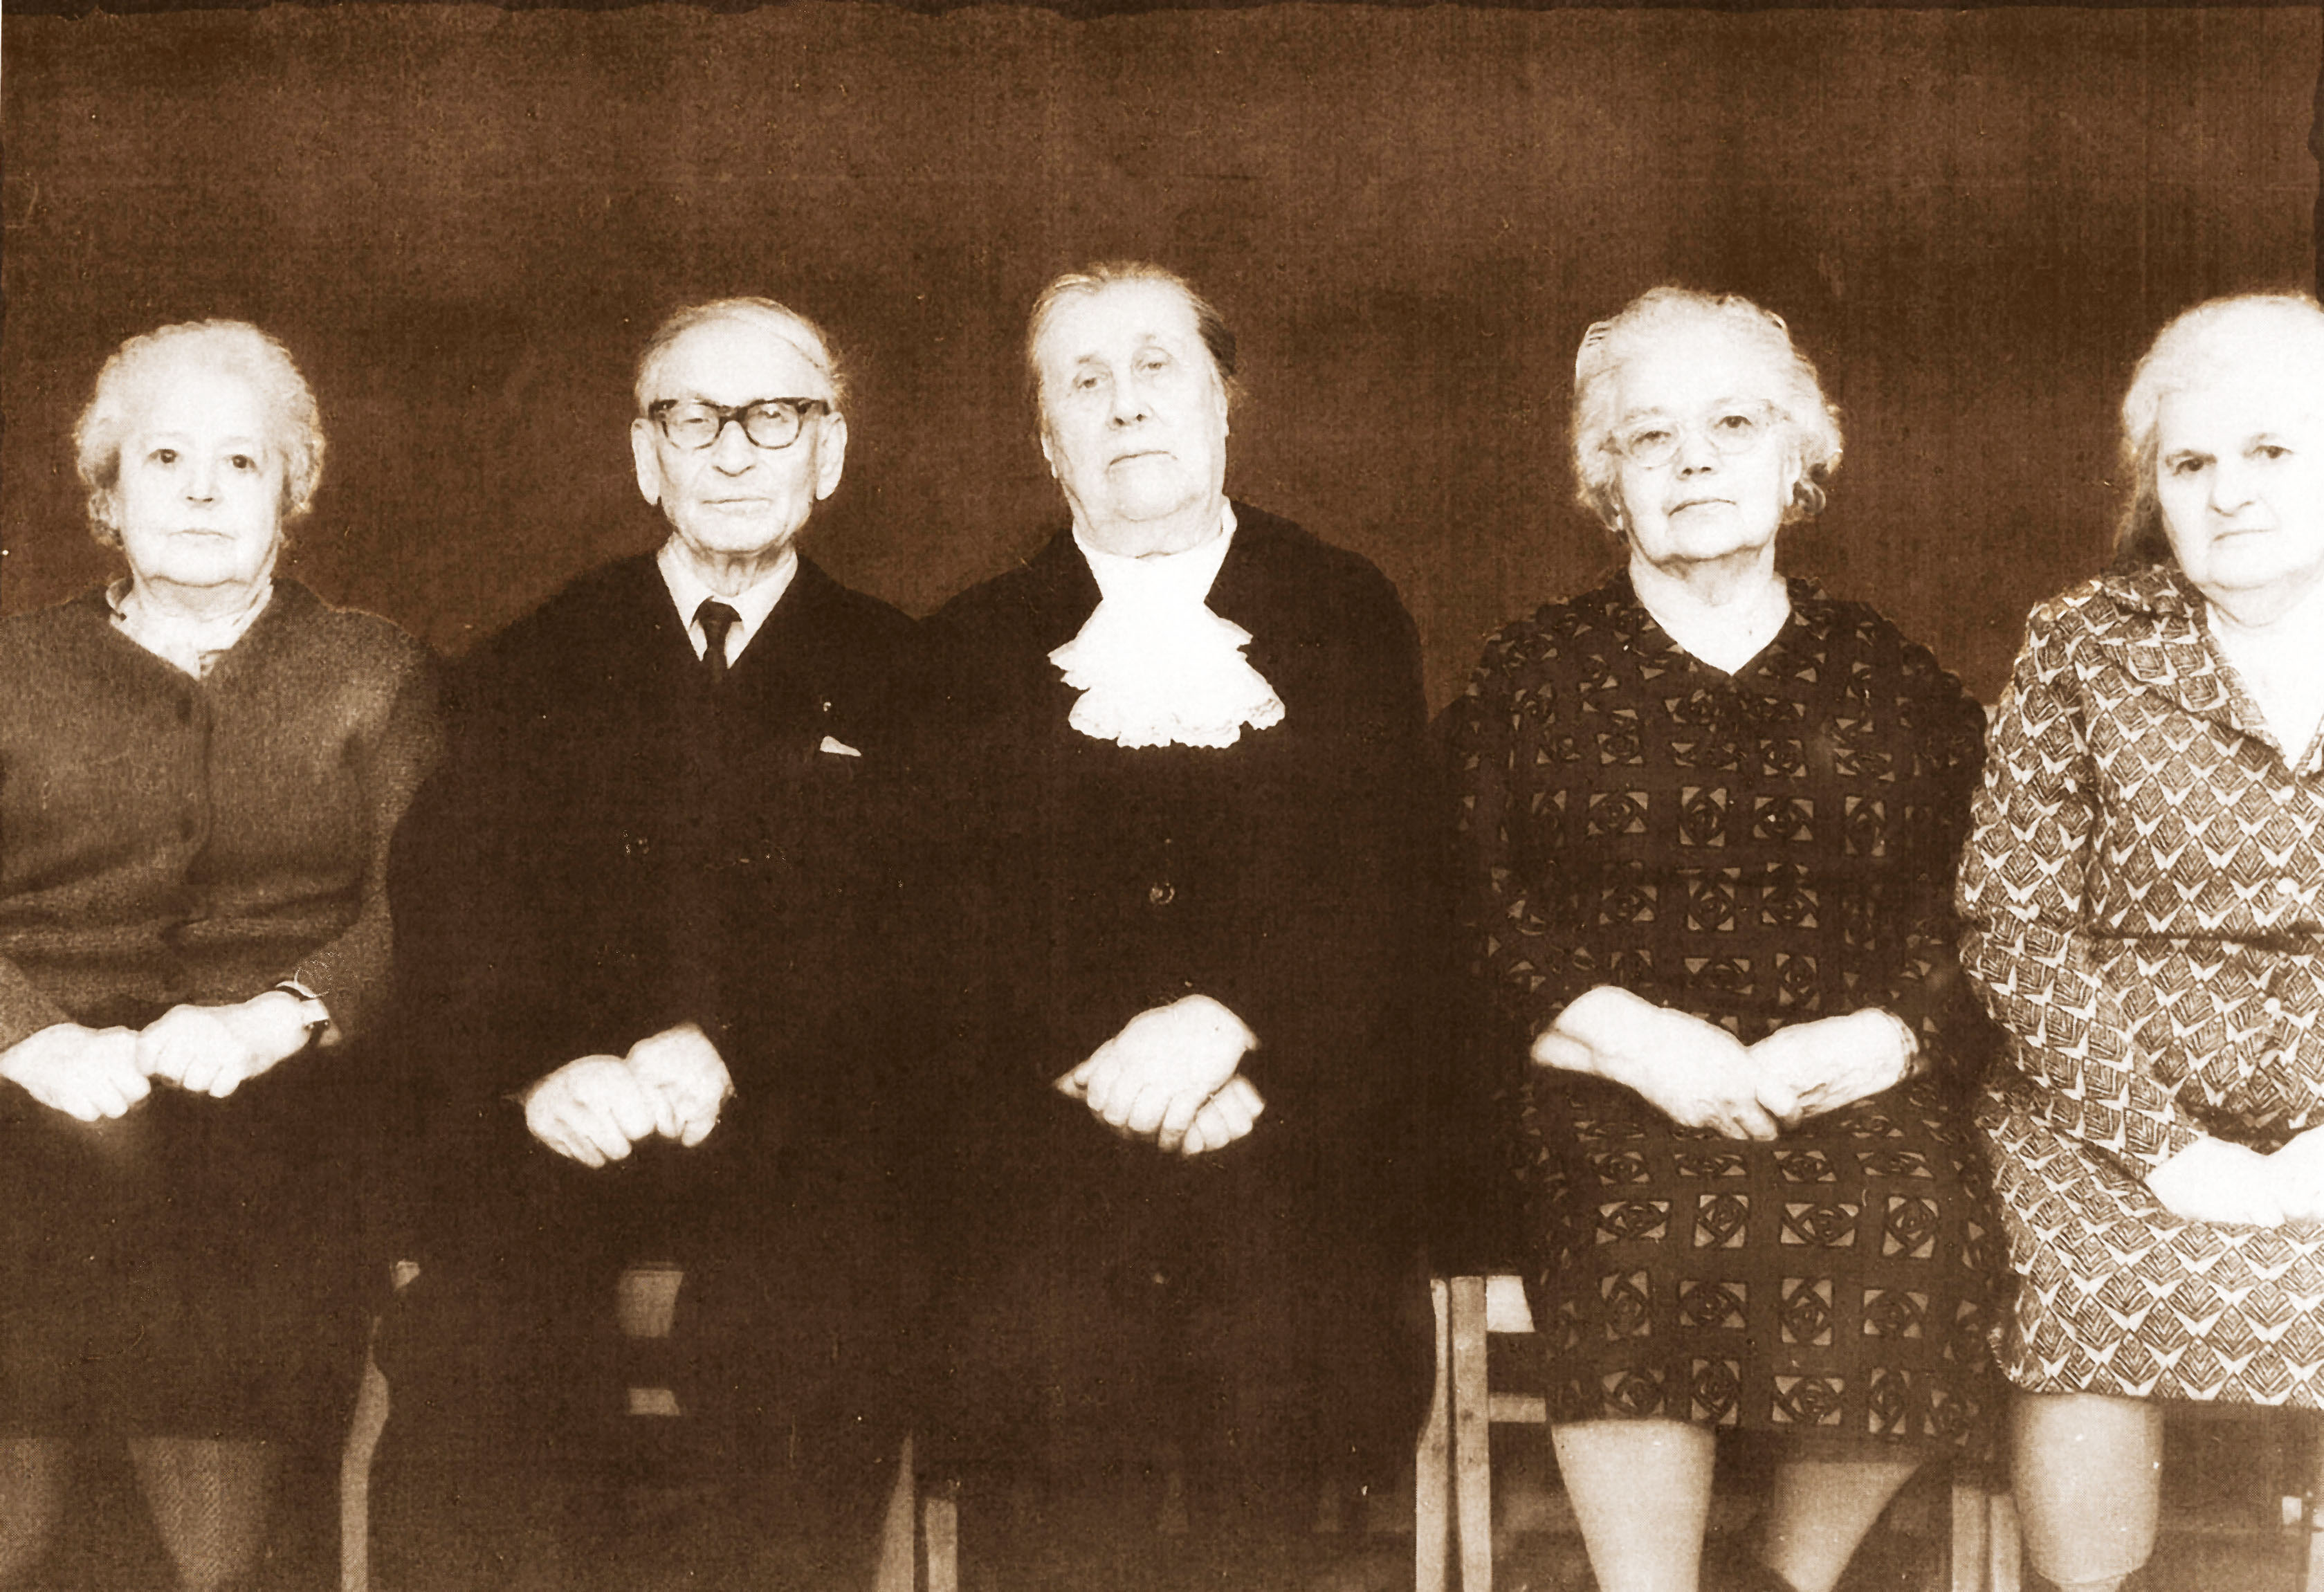
\includegraphics[width=7cm]{inc/3/1}
  \textit{\footnotesize{ Старший по Дому Меньшиков В. А. и его гвардия из <<первопоселенцев>>.}}
  \end{minipage}
\end{figure}

Предполагается, по-возможности, собрать и в систематизированном виде представить фактические данные и фотографии, в первую очередь относящиеся к <<первопоселенцам>> и семьям, въехавшим в дом в тридцатых-сороковых годах прошлого века.

Фотографии, представленные здесь, хорошо бы дополнить видом площади с <<живыми>> Красными воротами, а может быть и другими (к 2015 г. многое сделано).

Вводный раздел, кроме статьи авторов-составителей Т. В. Меньшиковой и К. Д. Варзар, мне кажется, хорошо бы дополнить отрывками об истории Дома из воспоминаний ветеранов (см. Приложения).

Если удастся добраться до архивных документов~-- старых домовых книг, будет дан полный поквартирный список <<первопоселенцев>> и <<второпоселенцев>> (30-е, 40-е годы).

Совет ветеранов провел большую работу по формированию, проверке и систематизации списков репрессированных жильцов Дома, в первую очередь в 1937~-- 1939 гг., и реабилитированных (часто~-- посмертно) в 1956 г. <<за отсутствием состава преступления>>. Соответствующие списки будут опубликованы в Альбоме.

Этот Совет долгие годы занят благородным делом~-- помогает ветеранам Великой Отечественной войны, рассказывает о них, отмечает с ними торжественные события и памятные даты, что, конечно же, тоже будет отражено в Альбоме. Особая страница будет посвящена погибшим на этой войне. Не будут забыты и герои тыла.

Хорошо было бы по самостоятельной странице посвятить жильцам~-- семьям каждой из 97 квартир Дома. Но, к сожалению, через столько десятилетий раздобыть исчерпывающие данные, а особенно фото, невозможно.
Поэтому придется опубликовать только то, что удастся собрать. 

Ниже для примера в алфавитном порядке приведены данные\footnote{В Альбоме такие композиции будут размером 20 на 30 см.} о шести семьях: Варзаров, Кузнецовых, Меньшиковых, Миниксов, Моргуновых и Плоткиных.


\newgeometry{left=0mm, right=0mm, top=0mm, bottom=0mm}

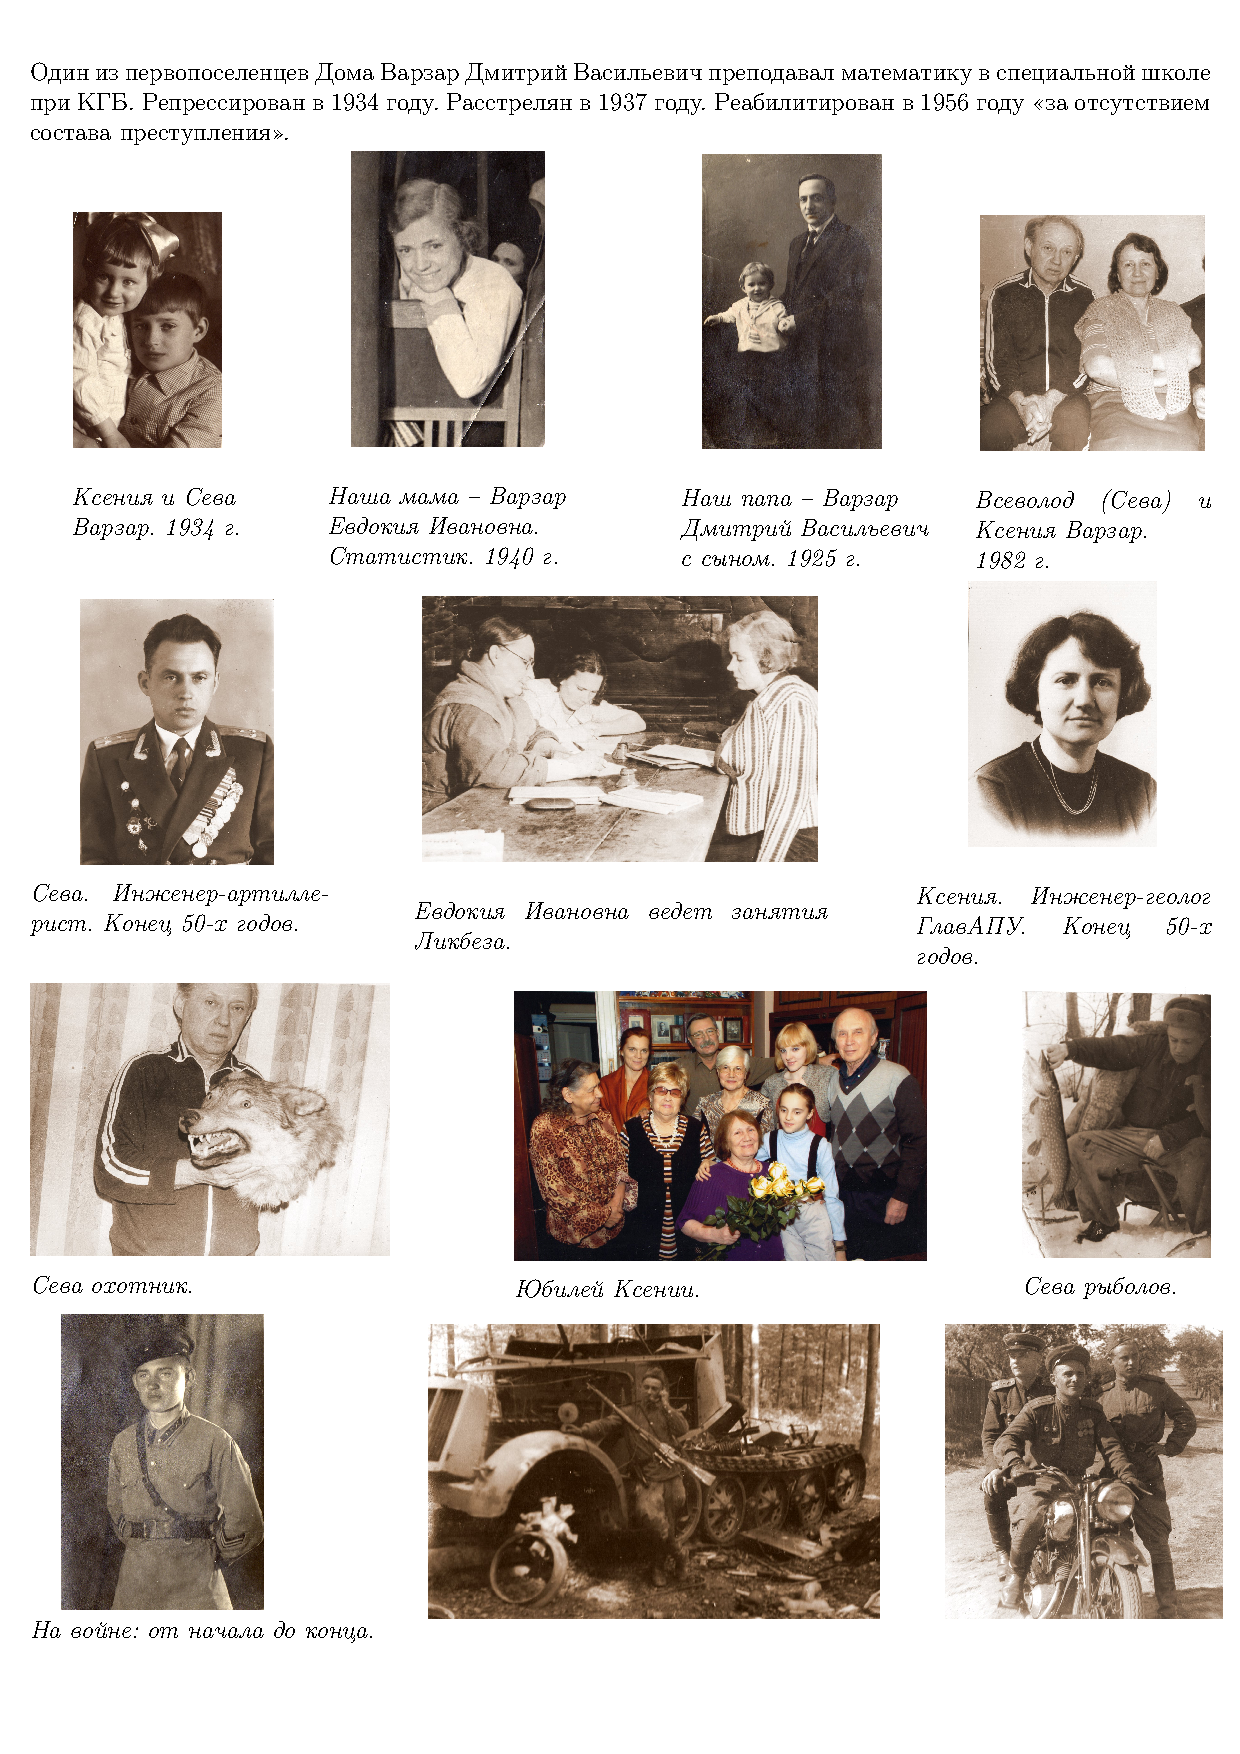
\includepdf[pages=-]{inc/varzar.pdf}

\noindent
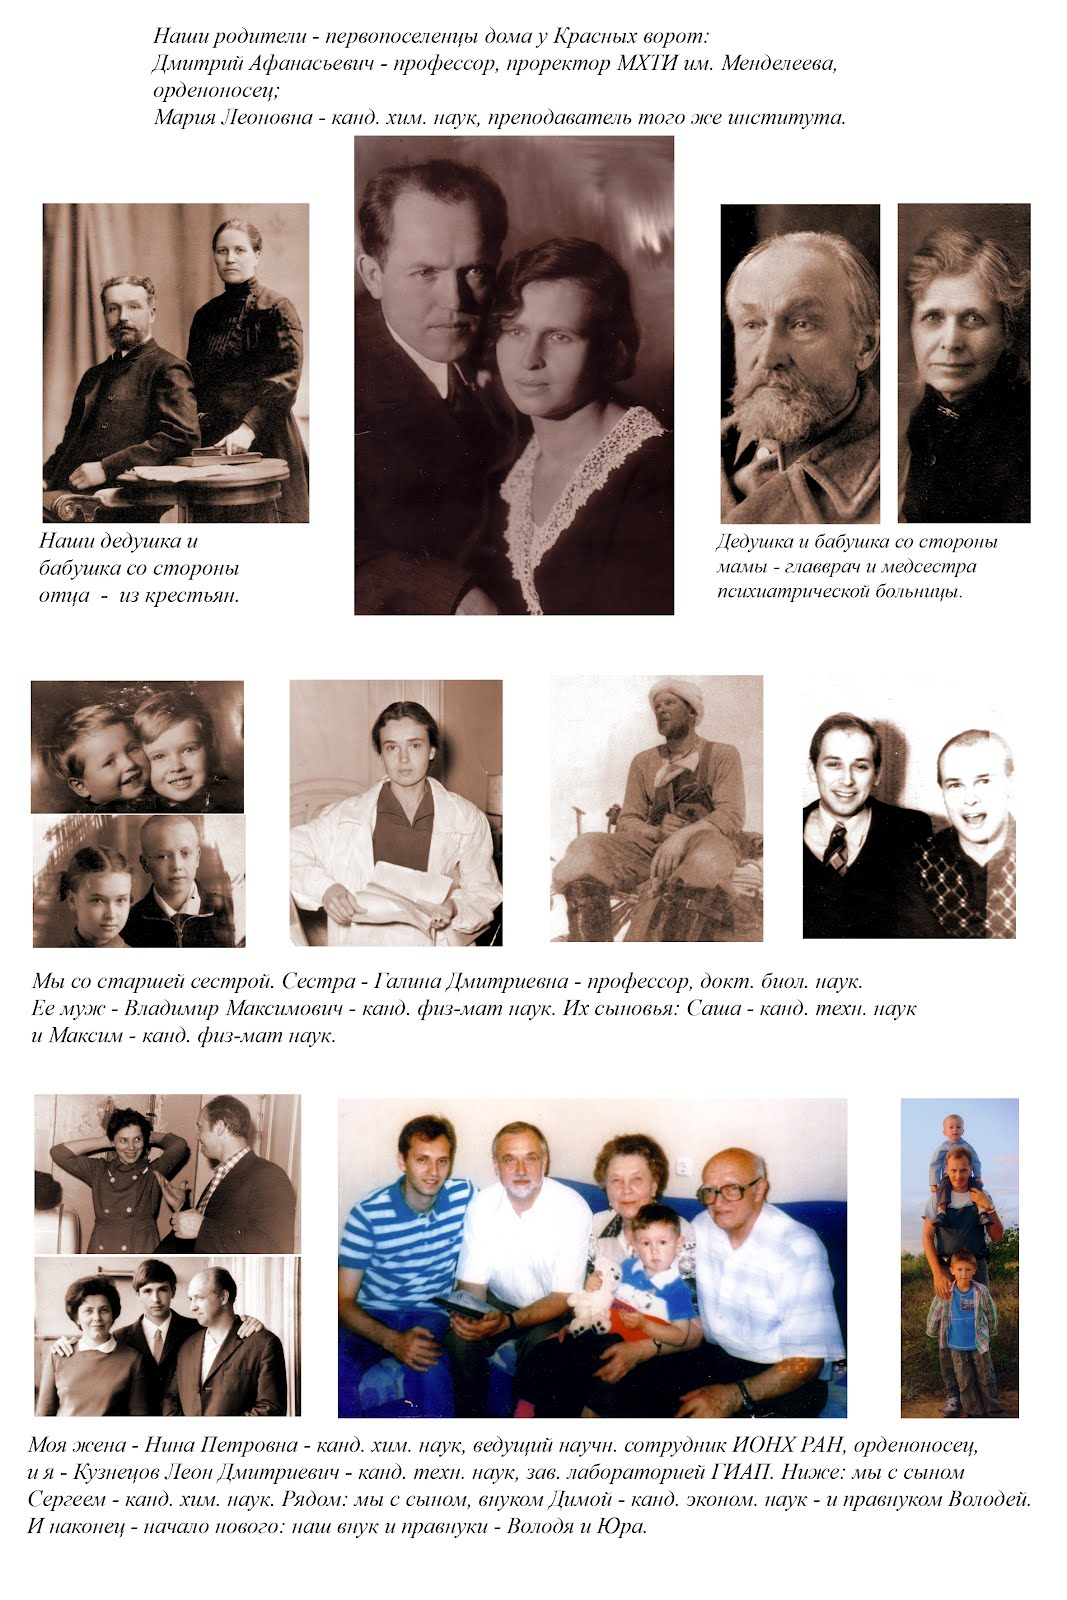
\includegraphics[height=\paperheight]{inc/kuznecovy}


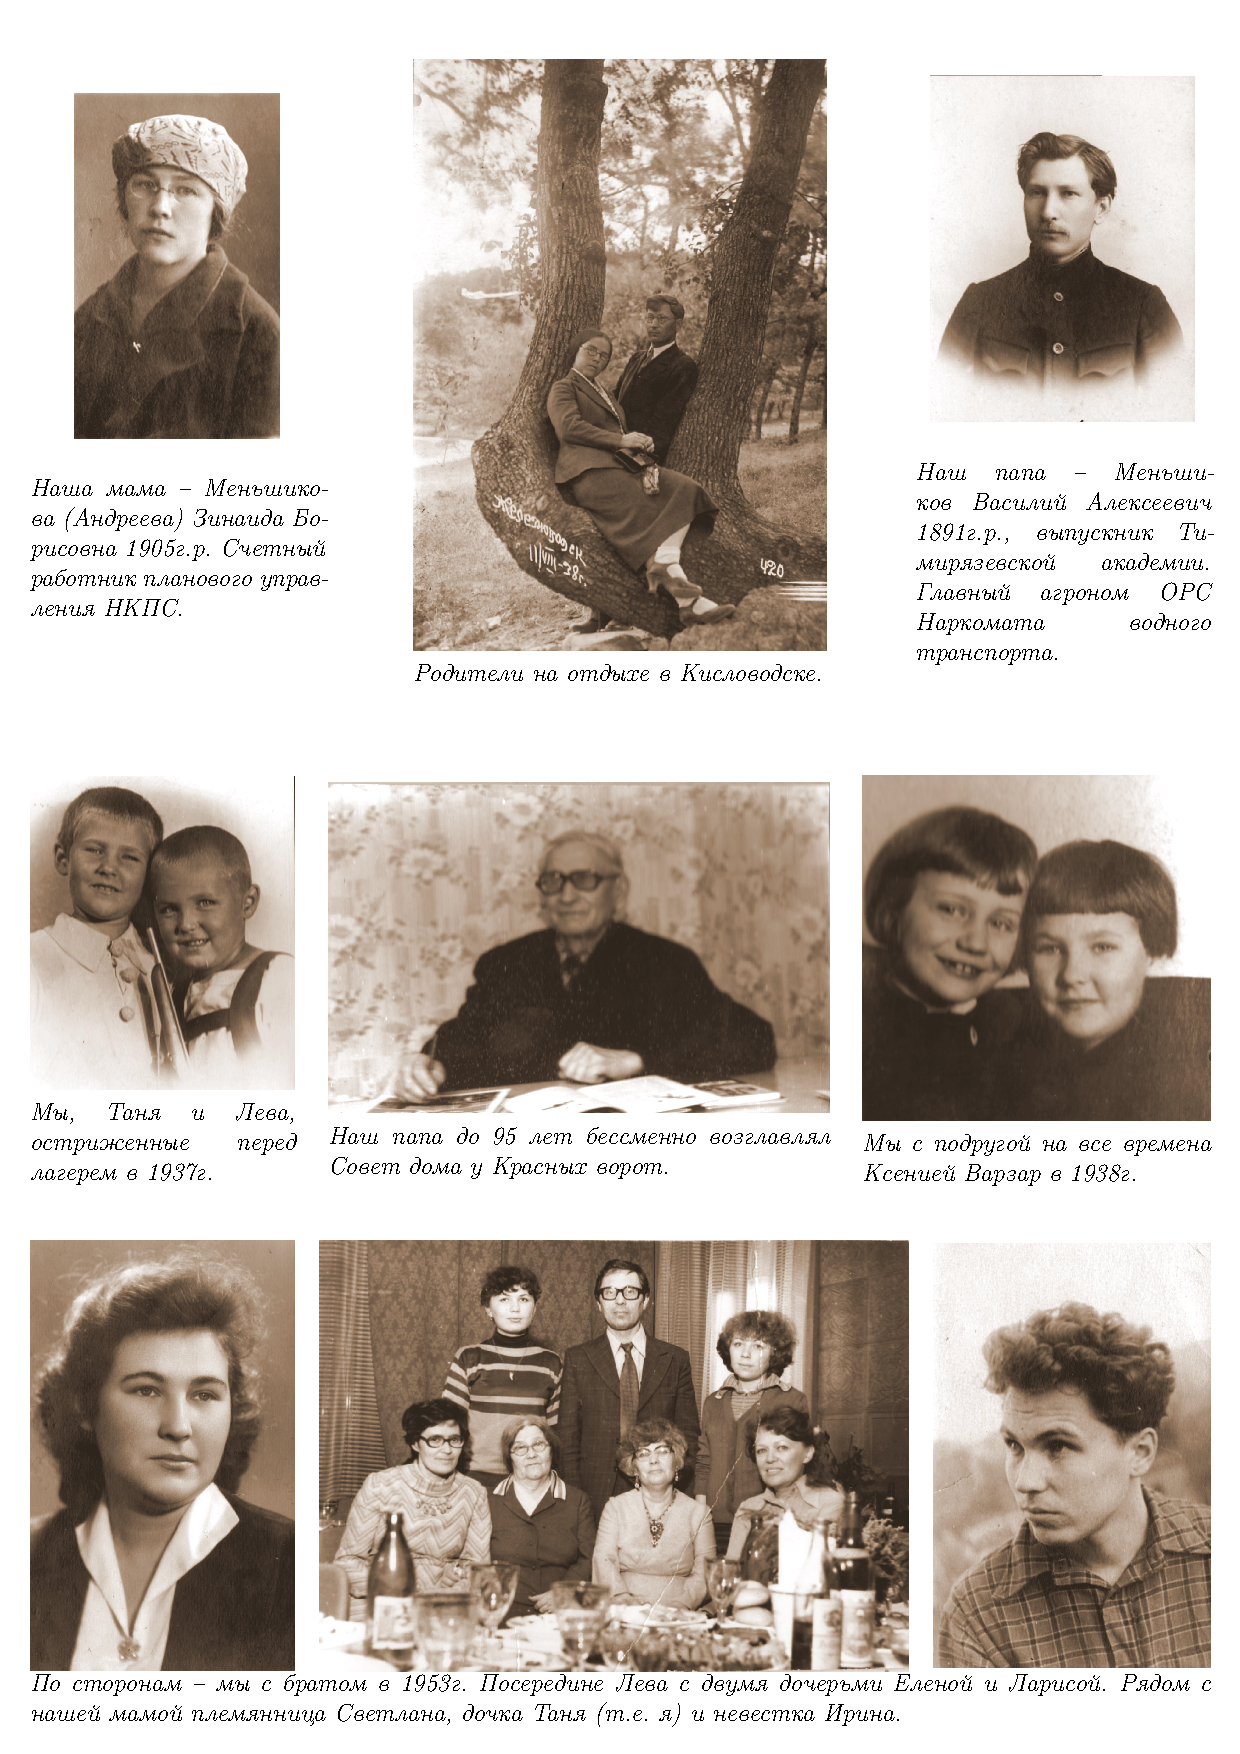
\includepdf[pages=-]{inc/menshekovy.pdf}


\begin{center}

\noindent
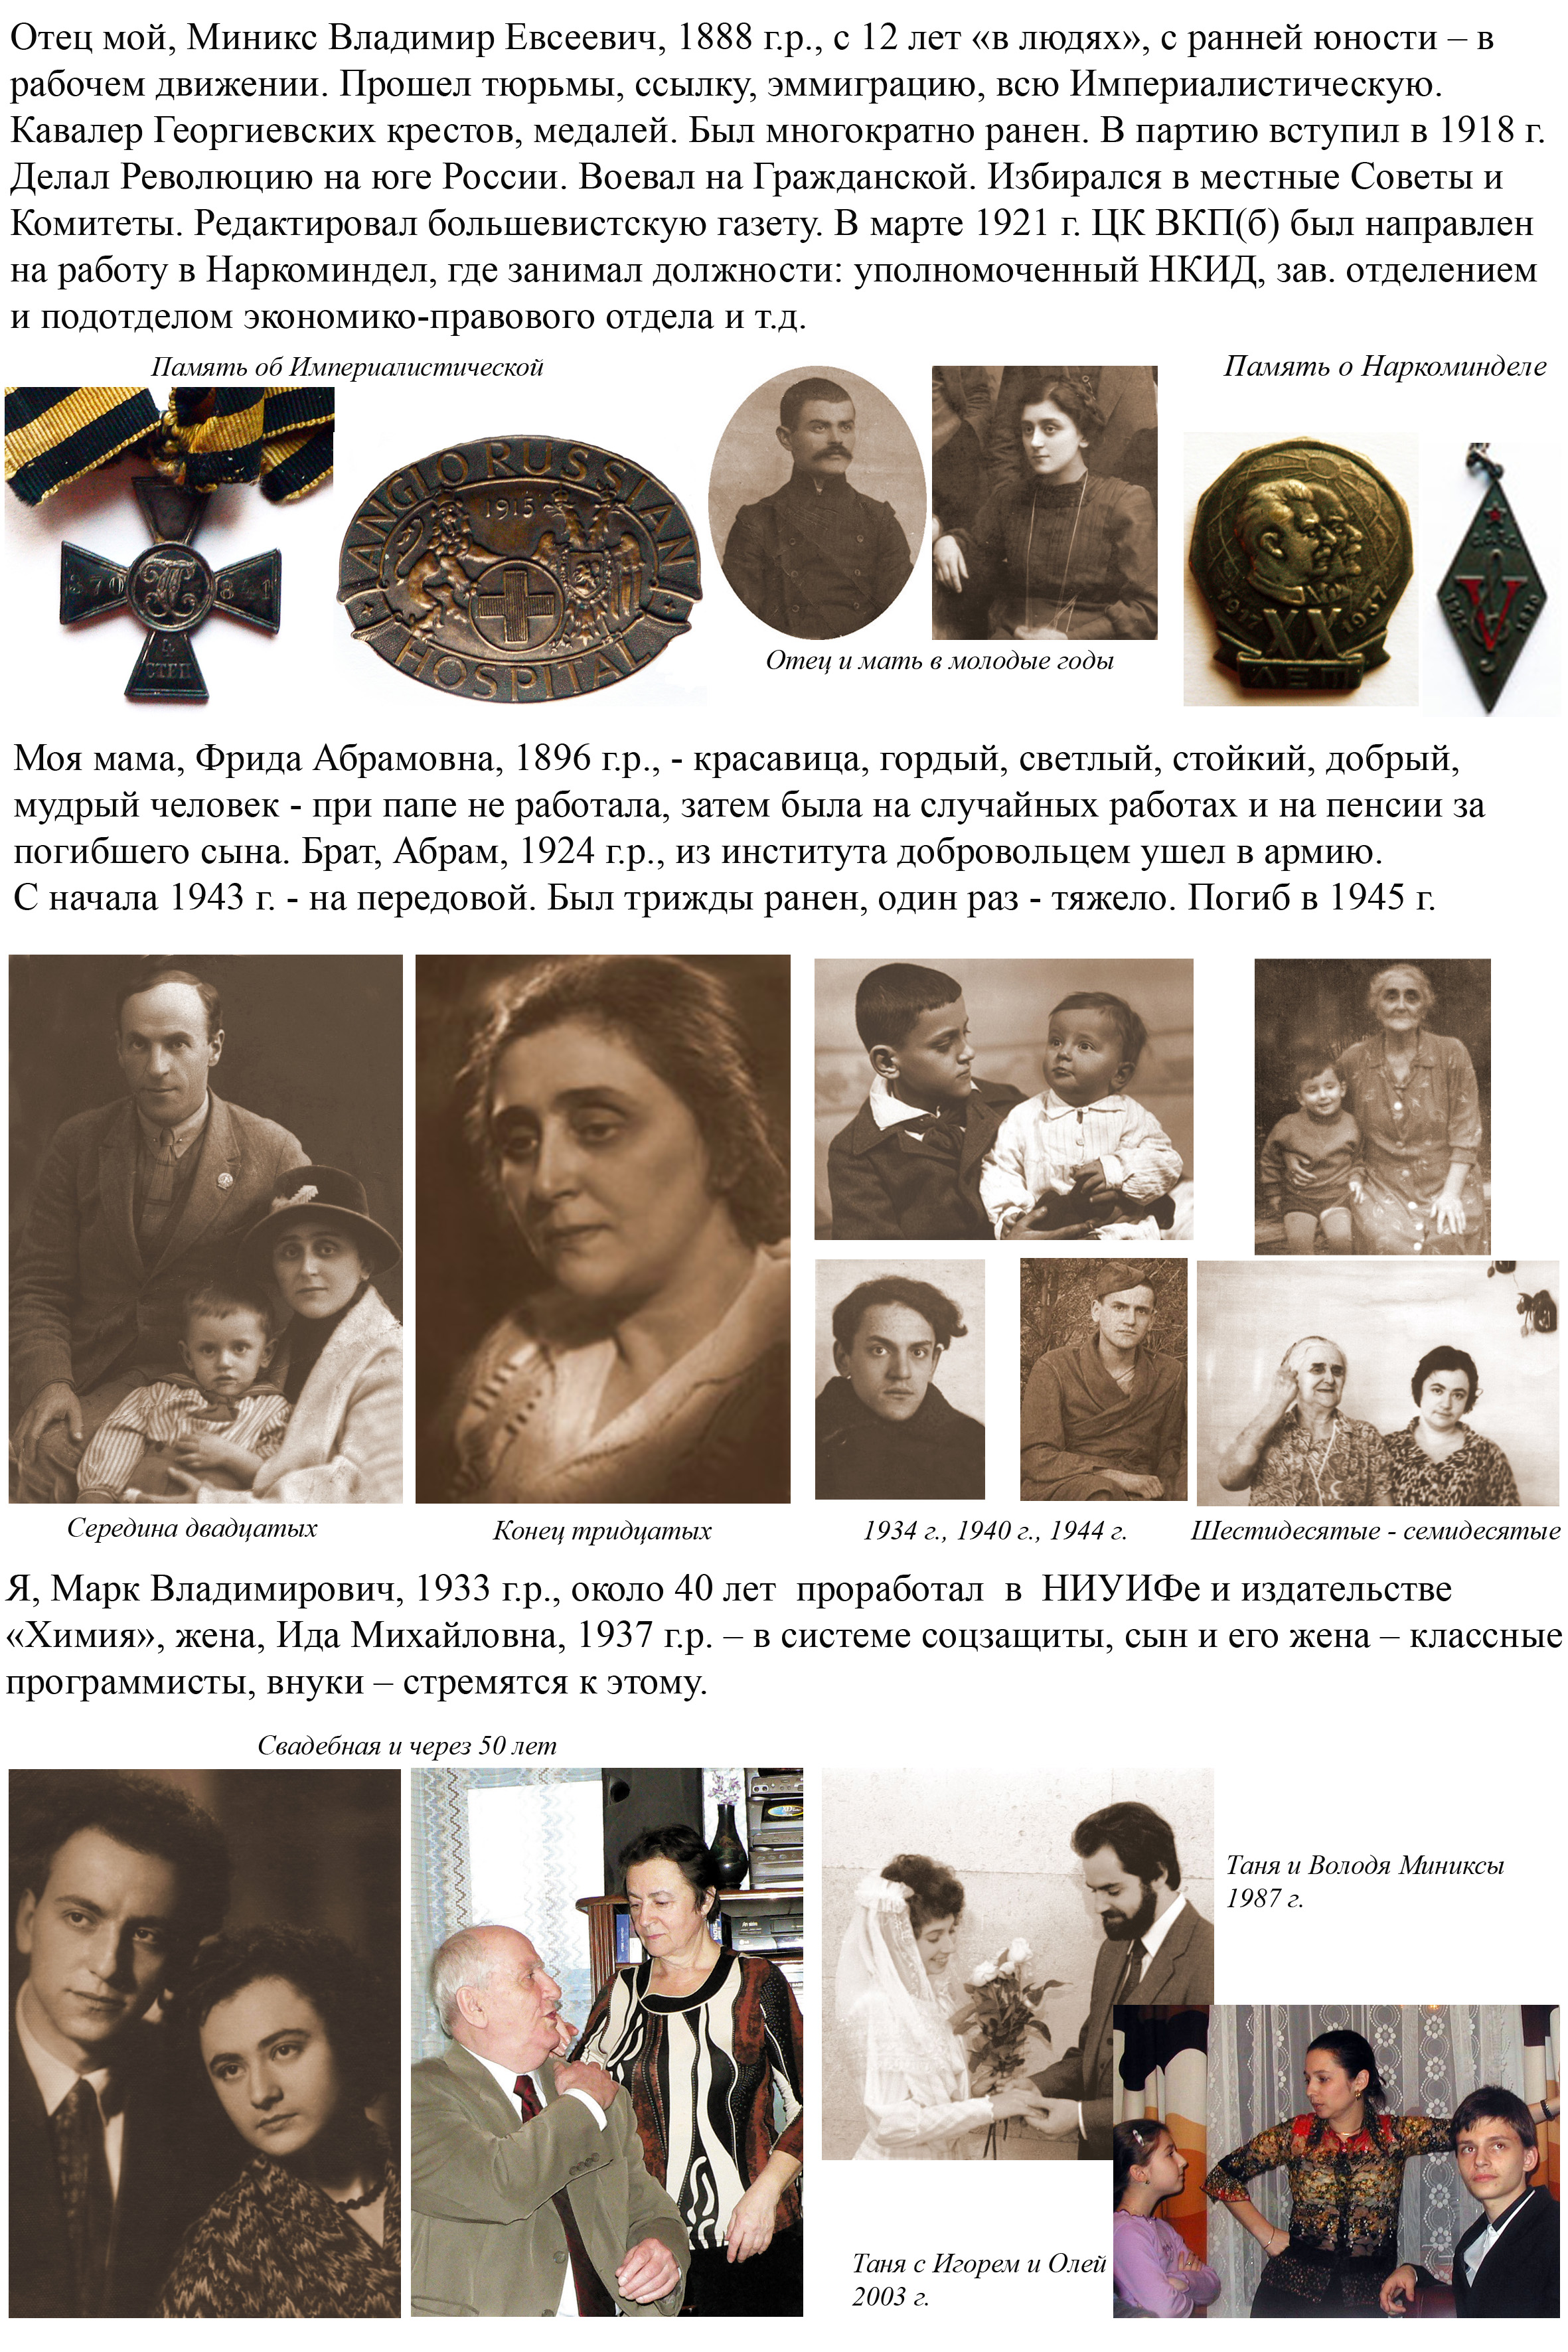
\includegraphics[height=\paperheight]{inc/minixy}

\noindent
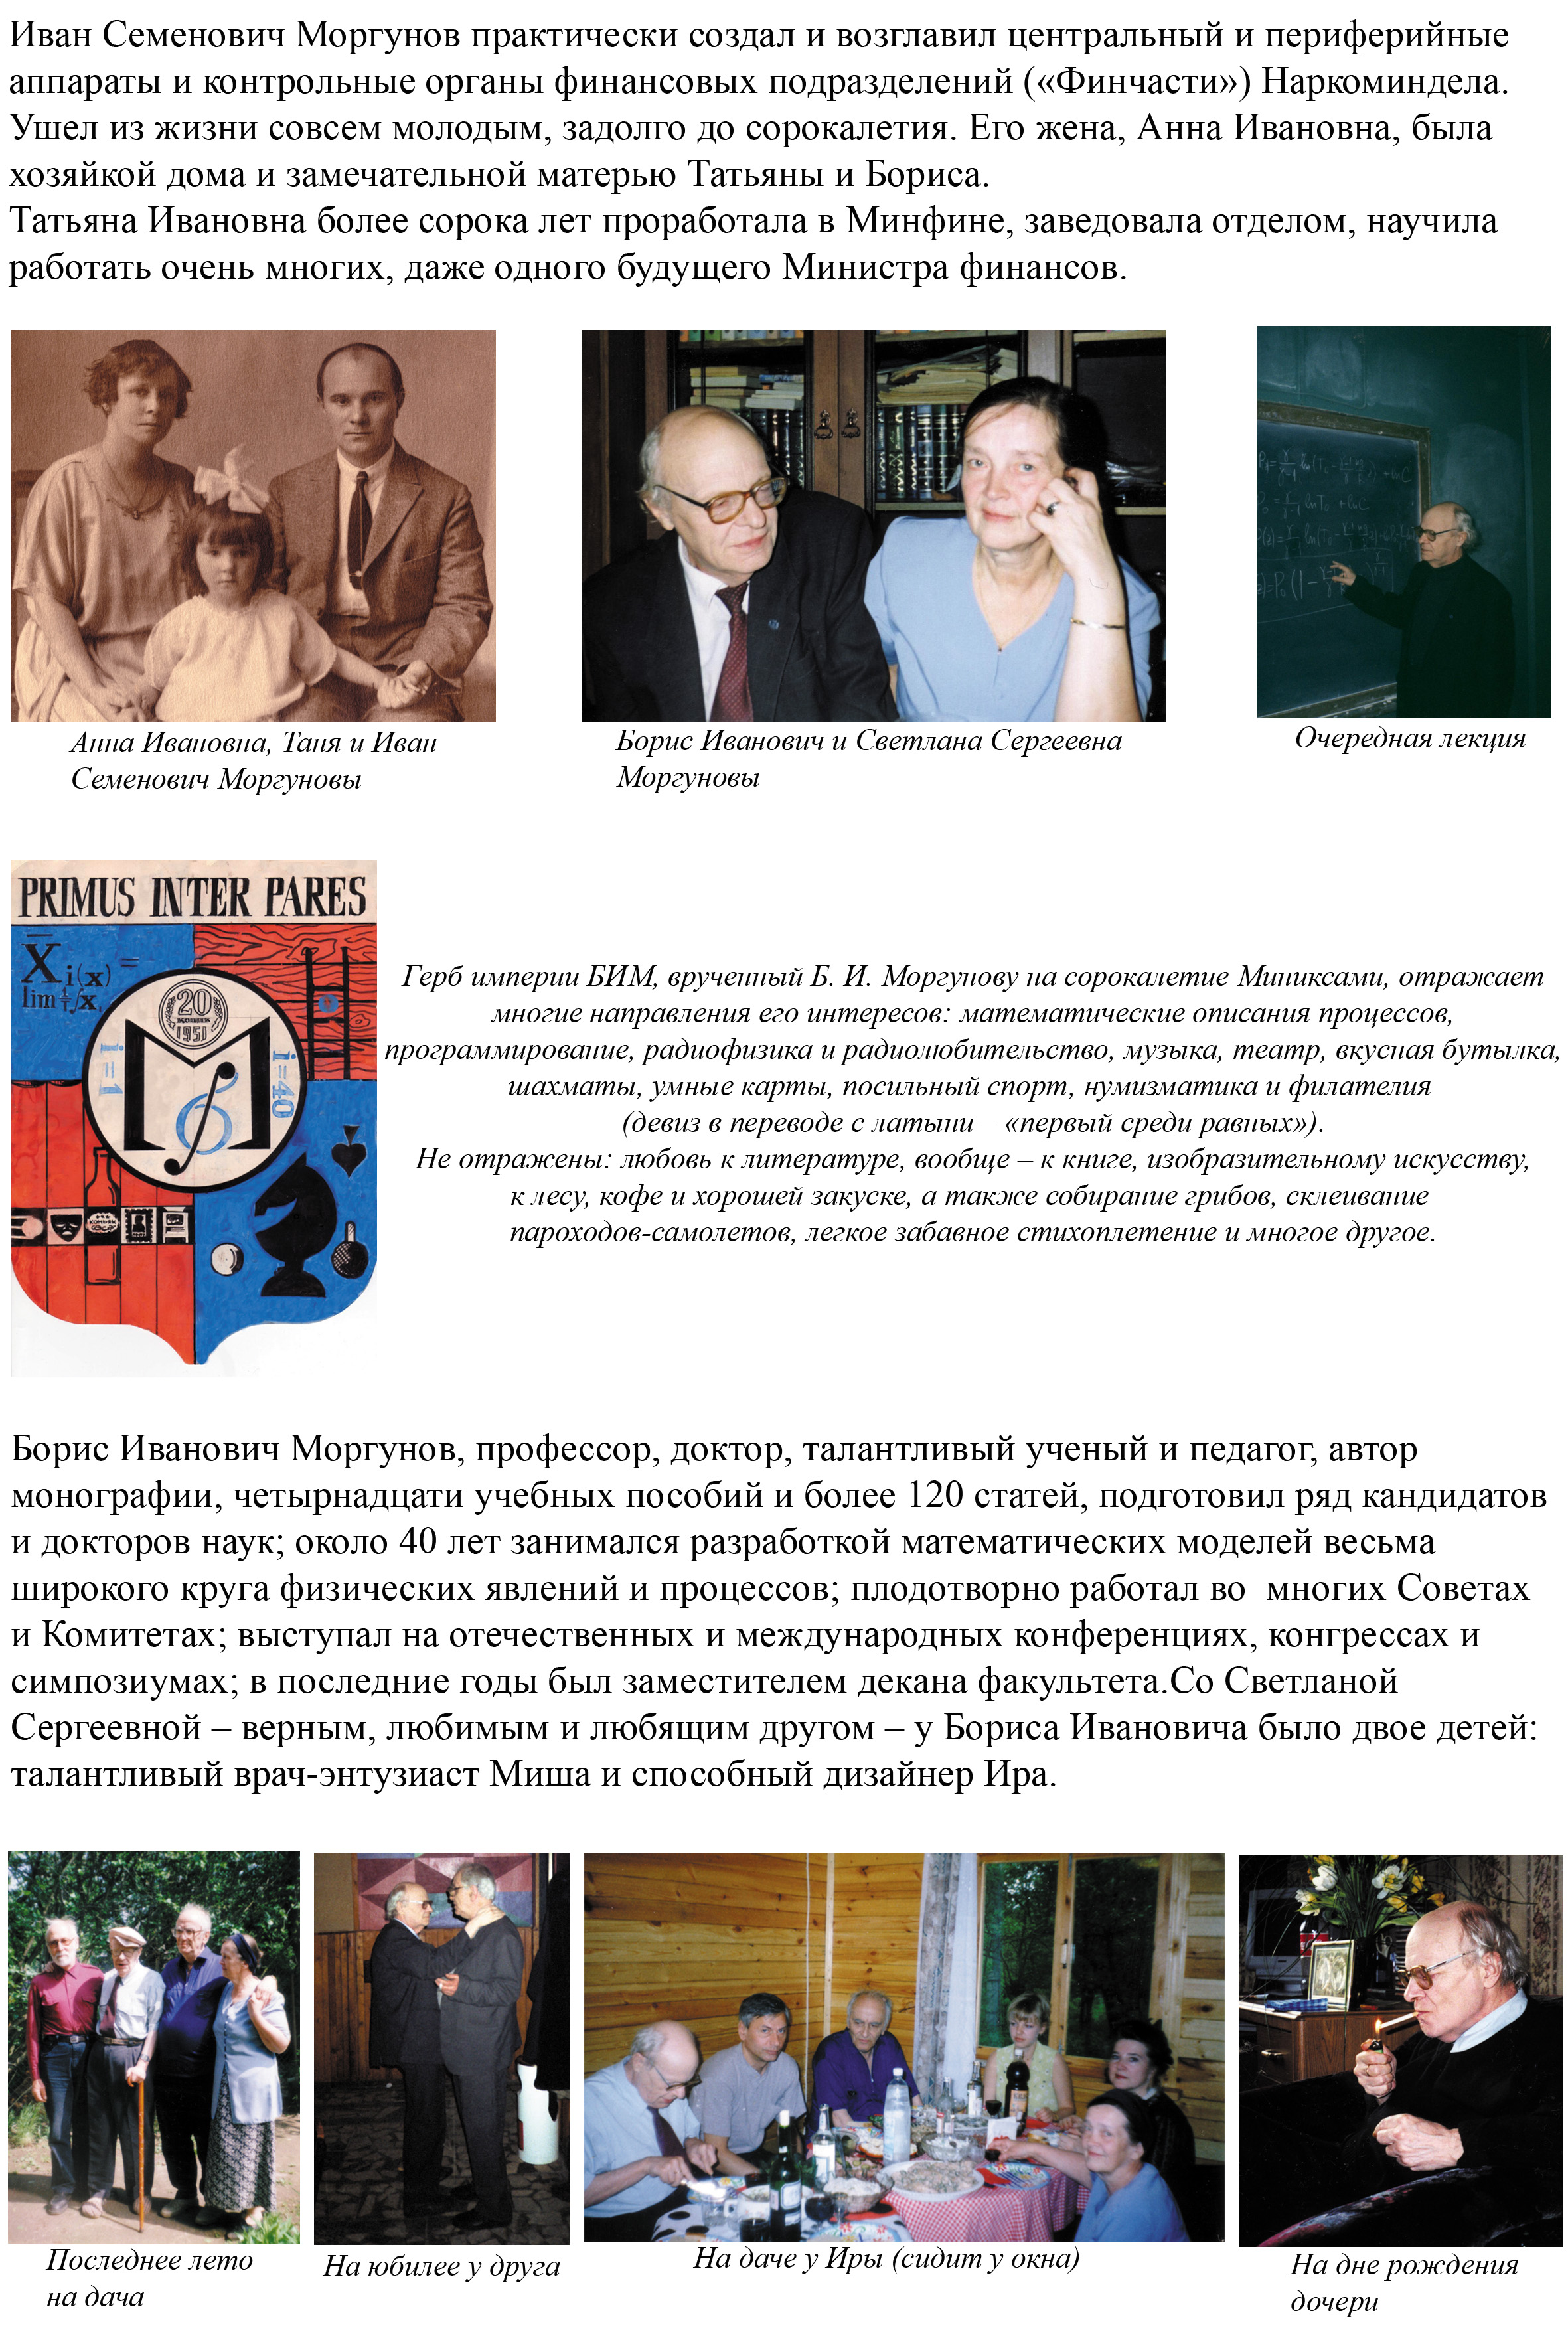
\includegraphics[height=\paperheight]{inc/morgunovy}

\noindent
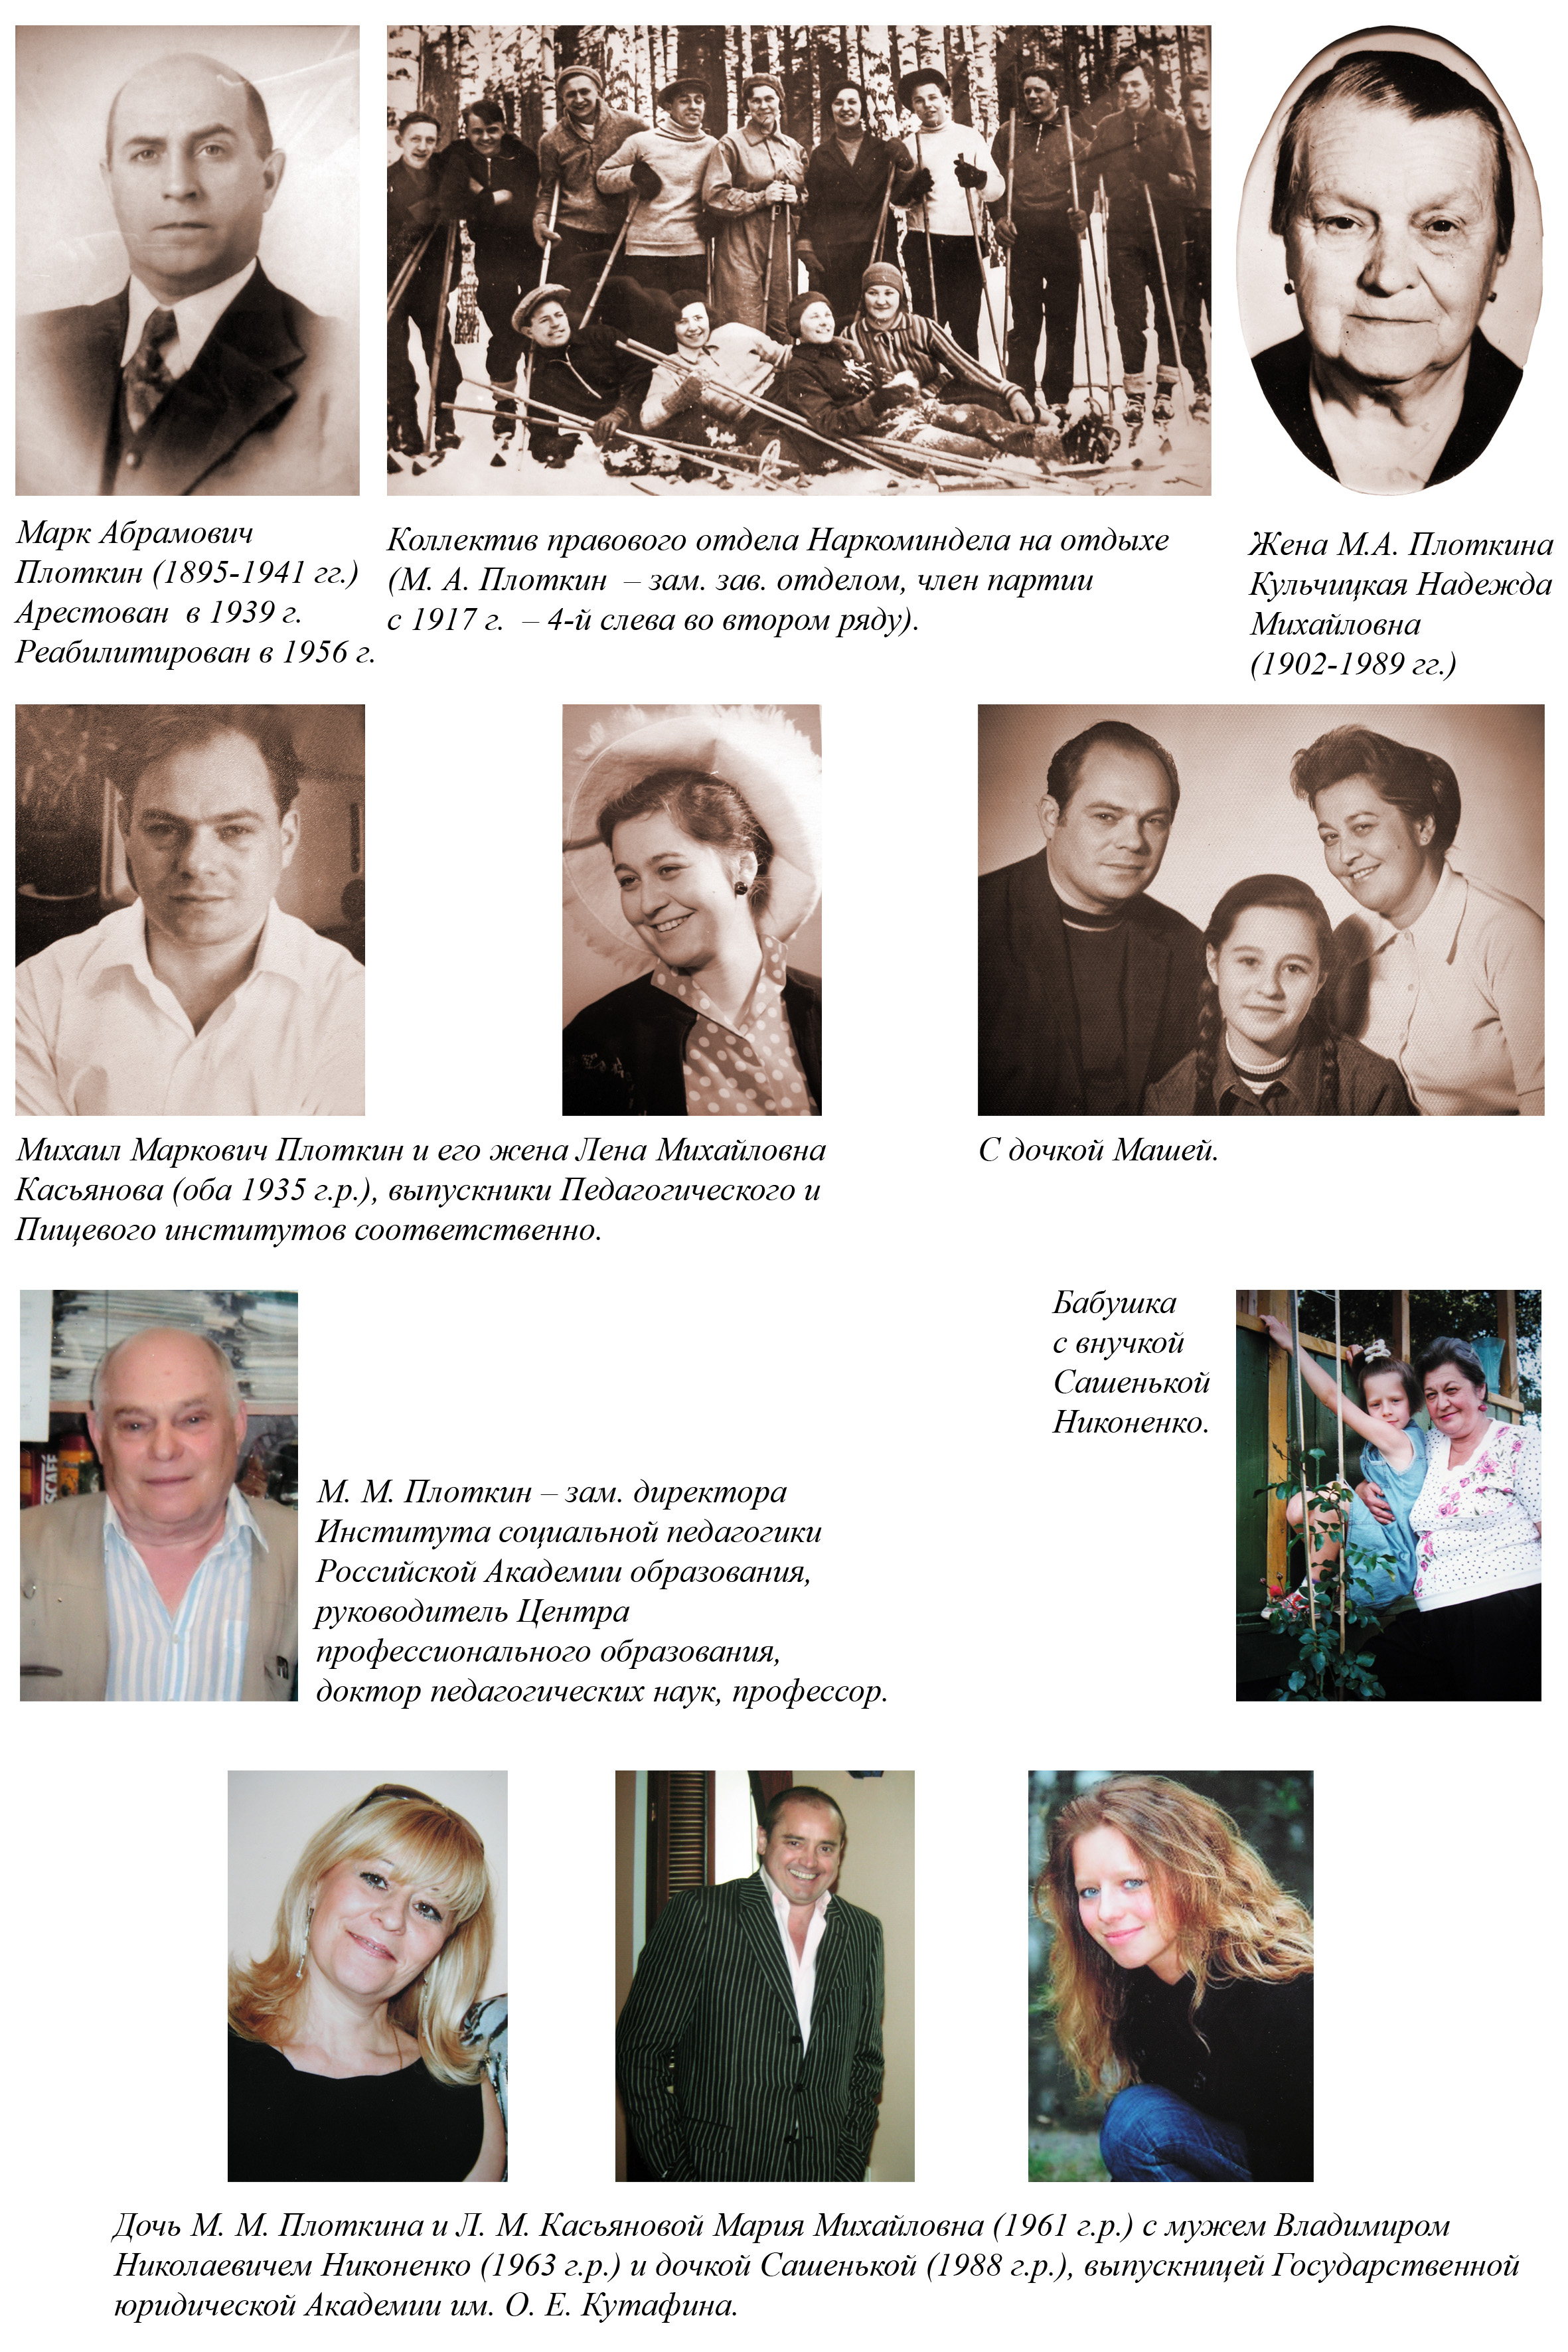
\includegraphics[height=\paperheight]{inc/plotkiny}

\end{center}

\restoregeometry

